\subsubsection{Middleware}
\subsubsubsection{Application - Middleware}
The communication protocol between application layer and middleware layer 
\paragraph{Fire and forget} 
It is a one-way message pattern (the service sends a message without expecting 
a response). Since the application and the middleware will reside on the same 
physical node we can assume that the communication is reliable, once a message 
is sent from the application layer it arrives to the middleware layer and 
viceversa. The asynchronous communication decouples (when possible) 
the computation of the application from the computation of the middleware 
and viceversa. The standard interfaces for communication 
implemented by application layer and middleware layer enables the use of 
heterogeneous technologies for each one. Defining a standard interface 
is fundamental to abstract from the underlying technologies (implementation).

\subsubsubsection{Middleware - Middleware}

The communication between the middleware layers implies the design of different 
services. Taking into account the distributed nature of the system we have 
studied specific solutions for each service, the ideas applied come from 
well known patterns used in distributed systems:
\begin{itemize}
  \item Lamport logical clocks: in a distributed system we are interested 
in the logical sequence of the events and not the wall clock time which is 
impossible to know perfectly and could lead to synchronization errors;
  \item Lamport timestamps algorithm\footnote{Leslie Lamport \textit{Time, 
clocks, and the ordering of events in a distributed system}, ACM 21, 
pp. 558-565, July 1978}: this algorithm contains the keystone 
of each distributed service which implies a form of synchronization 
between parties;
  \item Bully algorithm: this algorithm is used in the first part of the 
shutdown process. It works dynamically and implies the election of a master 
node. 
\end{itemize}

\subsubsubsection{Election Protocol}
This protocol tries to resolve the problem of the global consensus in a distributed system through the election
of a coordinator node, this version tries to improve the efficiency of the bully algorithm through the notification in case of a crash detection. The protocol assumption are as follows:
\begin{itemize}
  \item Each node knows the total number of nodes in the system (this information is gained during the censuns process);
  \item Each node has a different priority/ID;
  \item There is no natural time bound for this process to complete. A user-defined bound could be setted as system parameter before starting the process;
  \item At the end of the process the highest priority/ID (active) node is elected as coordinator.
\end{itemize}
The rules of the protocol are as follows:
\begin{enumerate}
  \item A node N sends an \textit{election} message to each node M with \textit{higher} priority/ID than him;
  \item N sets a timeout for each node M. If the timeout elapses then the receiver D is considered dead;
  \item M\footnote{M is any node with higher priority/ID than N} replies with an \textit{ok} message, which means that M is ready to continue the election process;
  \item M repeats the points 1. and 2. until the highest priority/ID node H is reached;
  \item If N has detected at least one dead node then N sends a \textit{crash} message \textit{with dead node IDs} to M;
  \item M stops waiting for the nodes reported in the \textit{crash} message;
  \item When H is reached there isn't any other active node with higher priority/ID than him;
  \item H sends a \textit{coordinator} message to each active node K;
  \item Each node K replies with an \textit{ack} message to H;
  \item When the last node K has replied H has received all \textit{ack} messages thus completing the election process.
\end{enumerate}
Note and side cases:
\begin{itemize}
  \item If none of the M nodes reply then N elects himself as coordinator sending a \textit{coordinator} message to each L node which has lower priority/ID than him;
  \item If the dead node is the highest priority/ID node H and it restarts during the election process then it sends a \textit{coordinator} message to each active node L in the system. Each L possibly updates its coordinator state if the coordinator election isn't finished yet;
  \item If a possible coordinator node crashes during the election, the process restarts from another active node;
  \item This solution tries to reduce the timeout costs notifying higher priority/ID nodes when a dead node is detected;
  \item The communication is always between a lower priority node and a set of higher priority nodes, only during the \textit{coordinator} phase messages are broadcasted to all lower priority/ID nodes;
  \item The system has to freeze its state before starting the termination process, in this case all user inputs are ignored during the census and election processes.
\end{itemize}

\begin{figure}[H]
  \centering
  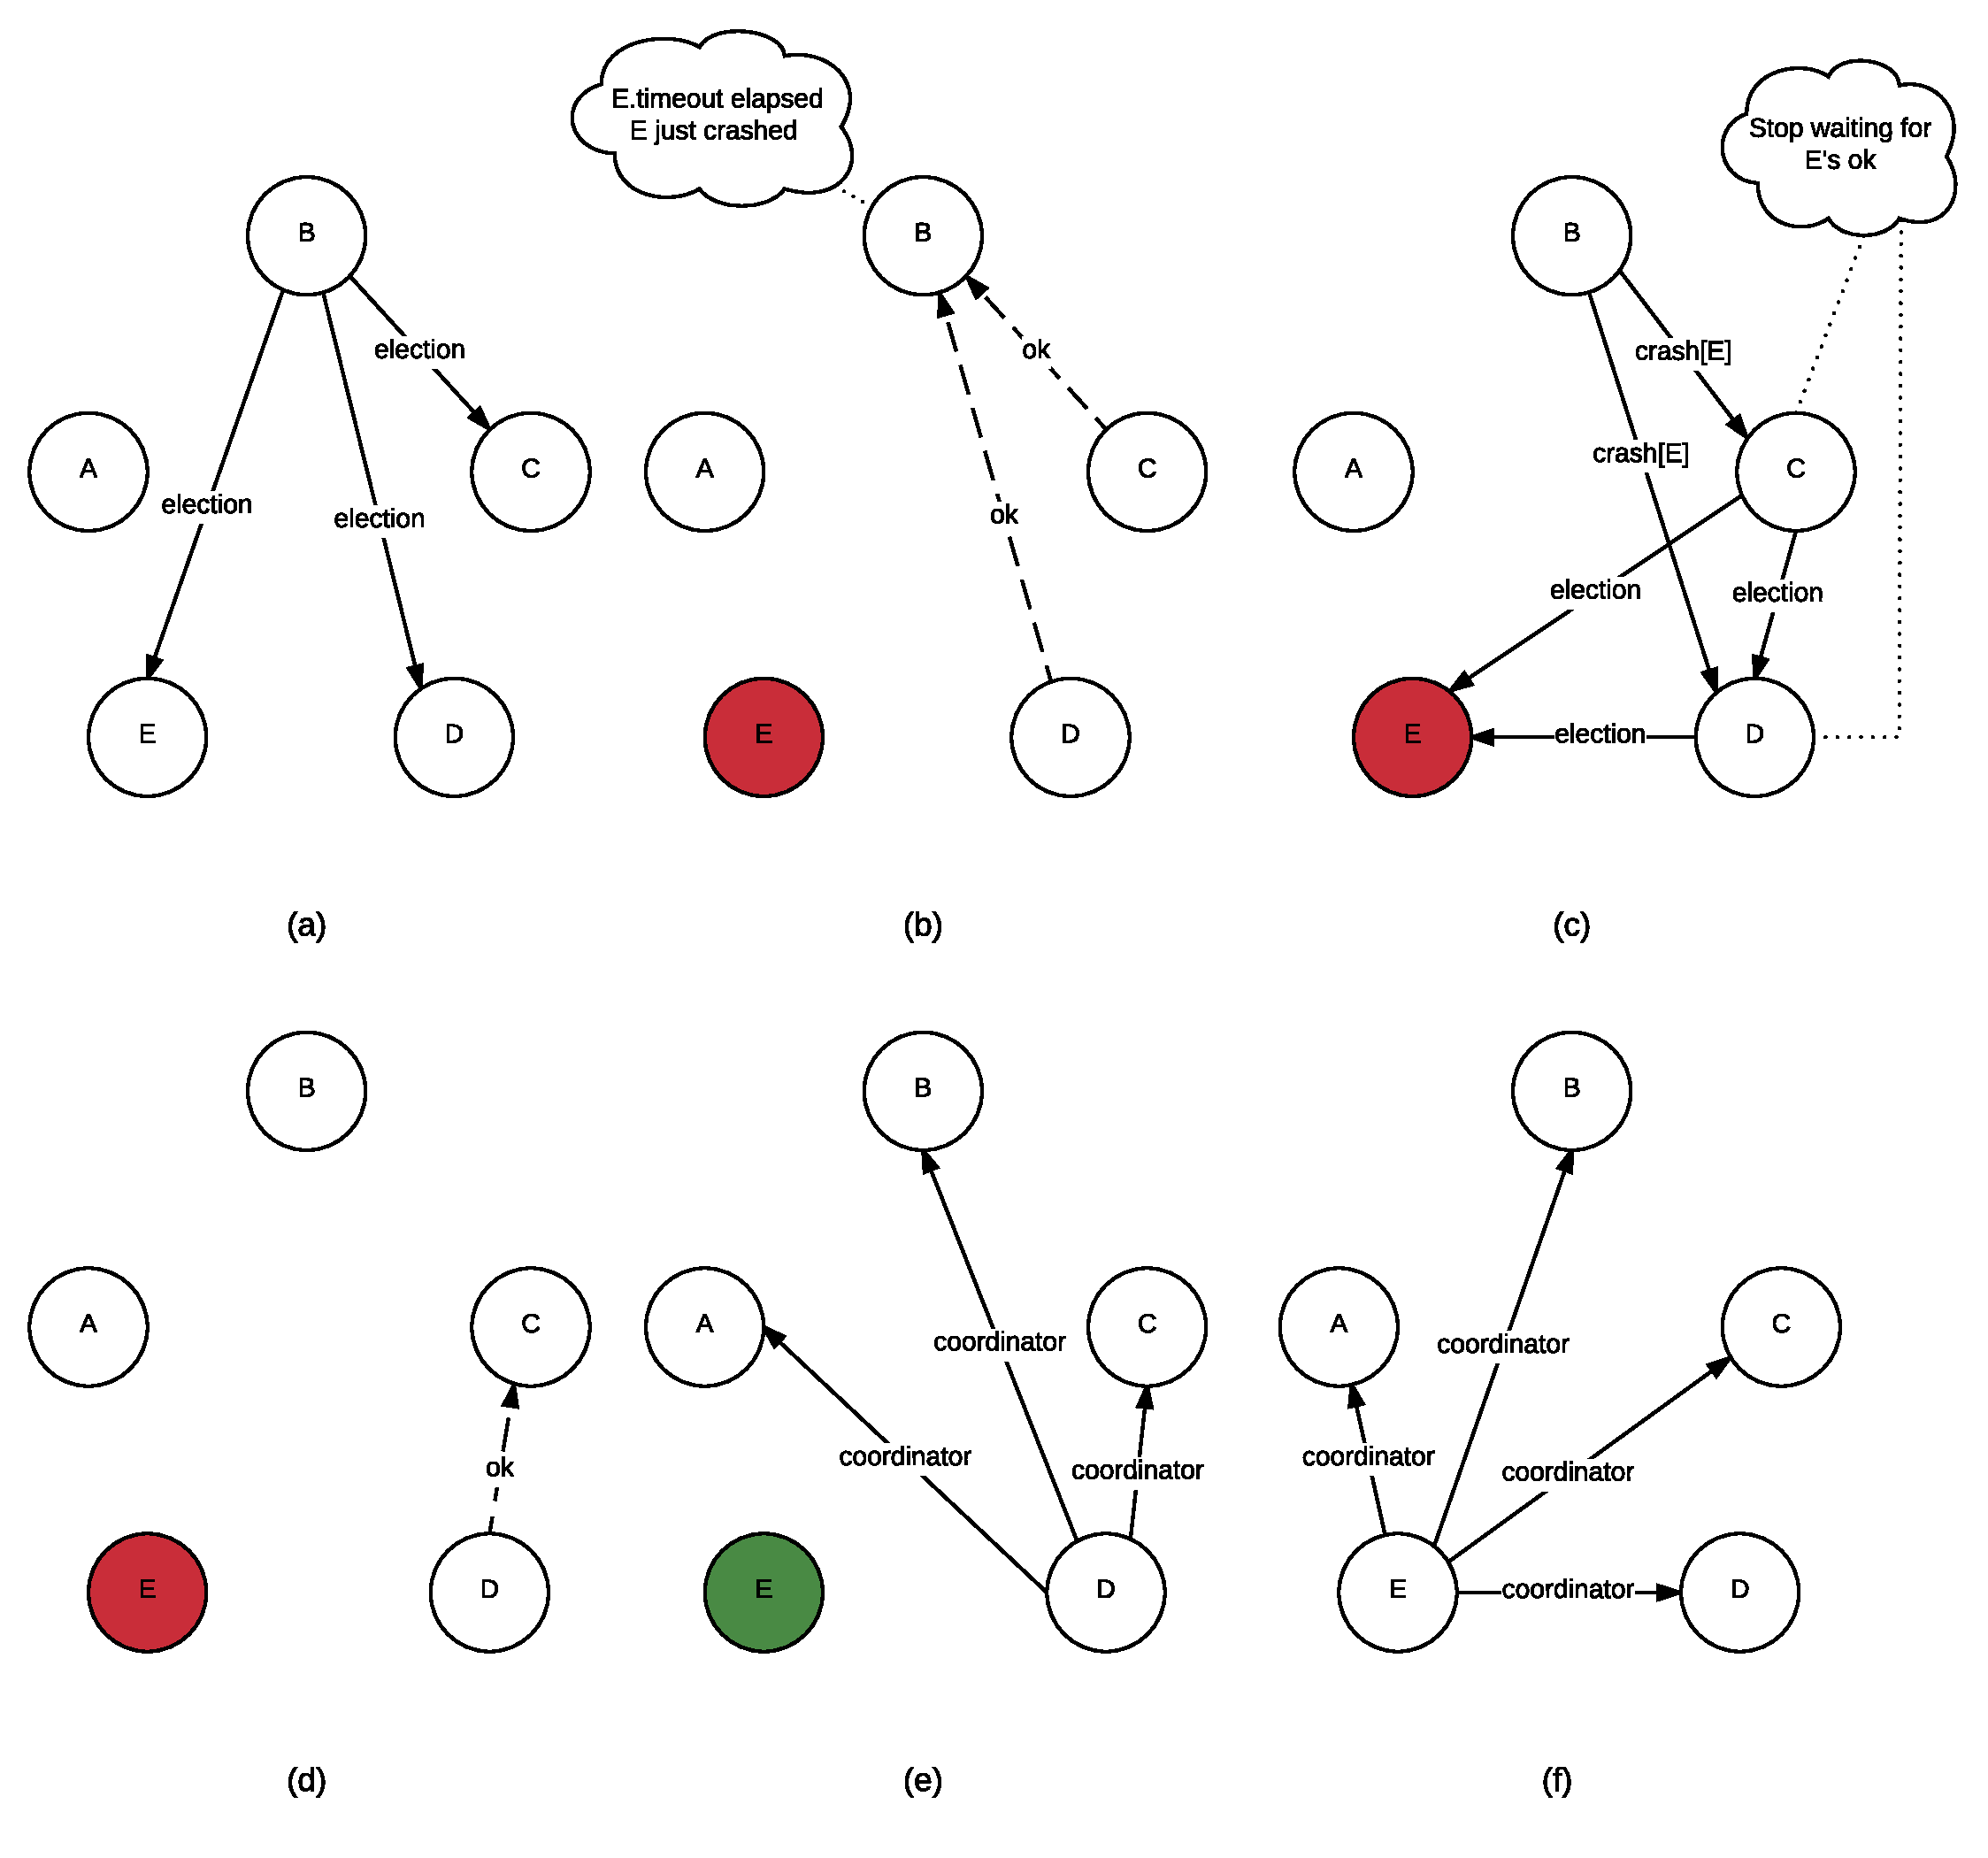
\includegraphics[width=\columnwidth]{sections/images/solution/election.pdf}
  \caption{Election protocol}
  \label{fig:election-protocol}
\end{figure}

\subsubsubsection{System Boostrap}
As pointed out in Problem Analysis (\ref{sec:pa-distribution}), the system has
to start neatly. Hence, we need to design a protocol in order to accomplish 
this goal.

The protocol is represented in figure \ref{fig:sys-bootstrap-protocol}, where:

\begin{itemize}
  \item A circle is a logical node which is composed of two layers:
    \begin{itemize}
      \item \textbf{MW}:  middleware layer
      \item \textbf{APP}: application layer
  \end{itemize}
    Since the middleware has to be application-independent, it only assumes 
    that the application layer exposes an interface through which it is 
    possible to start the application neatly;
  \item \textbf{Named arrow}: it represents a message that is sent from a 
logical node through another one with the name as its payload;
  \item \textbf{Number}: it represents the progress of the logical system clock 
during the bootstrap process.
\end{itemize}

\begin{figure}[H]
  \centering
  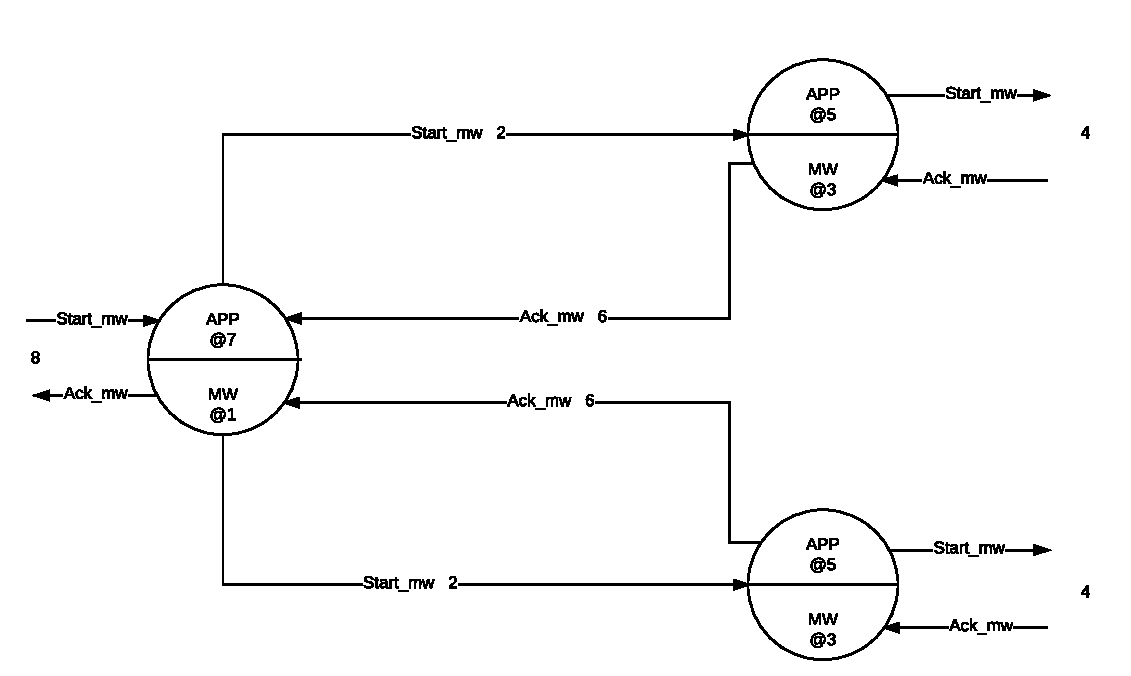
\includegraphics[width=\columnwidth]{sections/images/solution/bootstrap.pdf}
  \caption{System bootstrap protocol}
  \label{fig:sys-bootstrap-protocol}
\end{figure}

Assuming that a \texttt{Start\_mw} message arrives to a non-booted node (say
$l$) at time 0, the protocol is defined as follows:

\begin{enumerate}
  \item The leftmost node $l$ in figure \ref{fig:sys-bootstrap-protocol}
    starts its own middleware services.  
  \item $l$ sends a \texttt{Start\_mw} message to the set $S$ of all its
    neighbors. Clearly, if it was the first node in the system to receive
    \texttt{Start\_mw}, then it will be also the last node to complete the
    boot process.
  \item $l$ waits for each node in $S$ to complete the boot. $l$ waits for all
nodes in $S$ to send an \texttt{Ack\_mw} message back;
  \item The middleware MW of $l$ grants the application APP to start;
  \item $l$ then sends an \texttt{Ack\_mw} message back.
\end{enumerate}

As it can be seen in the figure, this behaviour is replicated recursively
by all nodes of the system. If a node has already been booted, then it only
sends \texttt{Ack\_mw} back.

\subsubsubsection{System Termination}
Also, the system has to shutdown neatly. Therefore we designed a protocol to
stop the entire system; please notice that this one could be seen as a
symmetric version of the System Bootstrap protocol.
% TODO: please check the sentence here above

The protocol is represented in figure \ref{fig:sys-termination-protocol}, where
the conventions are the same as the ones used in figure
\ref{fig:sys-bootstrap-protocol}.

\begin{figure}[H]
  \centering
  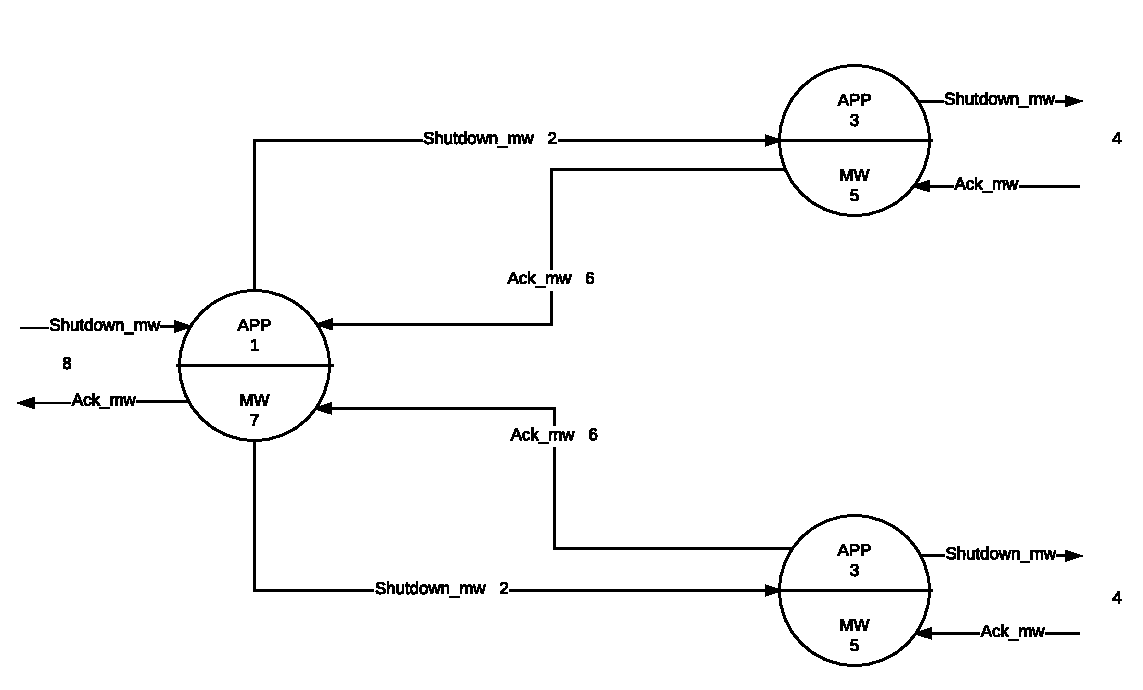
\includegraphics[width=\columnwidth]{sections/images/solution/termination.pdf}
  \caption{System termination protocol}
  \label{fig:sys-termination-protocol}
\end{figure}

Assuming that a \texttt{Shutdown\_mw} message arrives to a non-terminated node
$l$ (let it be the leftmost one in the picture) at time instant 0, the protocol
is defined as follows:

\begin{enumerate}
  \item The middleware MW of $l$ asks to terminate the application APP;
  \item $l$ sends a \texttt{Shutdown\_mw} message to the set
    $S$ of all the nodes it knows;
  \item $l$ waits for each node in $S$ to terminate, i.e. $l$ waits for all
    nodes in $S$ to send an \texttt{Ack\_mw} message back;
  \item $l$ stops its own middleware services;
  \item $l$ then sends an \texttt{Ack\_mw} message back.
\end{enumerate}

As it can be seen in the related figure, this behaviour is replicated
recursively by all nodes of the system. If a node has already terminated, then
it only sends \texttt{Ack\_mw} back.
